\section{Supporting online material}

\subsection{Supplementary code}

The \texttt{metafolio} \texttt{R} package and documentation.

\subsection{Supplementary figures}

\begin{figure}[htbp]
\centering
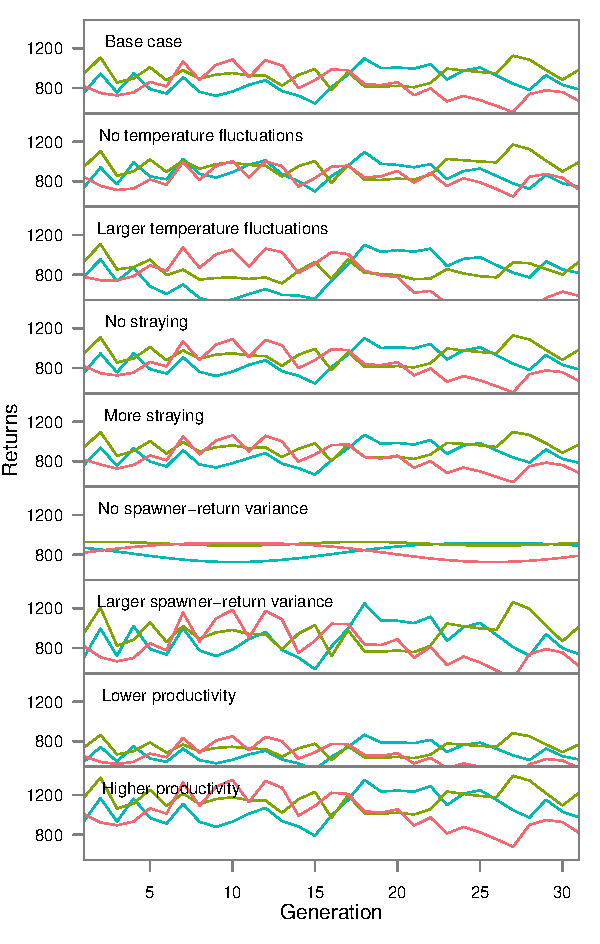
\includegraphics[width=4.0in]{../examples/figure/plot-various-options-ts-3pops.pdf}
\caption{The impact of increasing or decreasing various parameter values in the simulations. The different lines represent different salmon populations.}
\label{f:eg-sens}
\end{figure}

\clearpage

\begin{figure}[htbp]
\centering
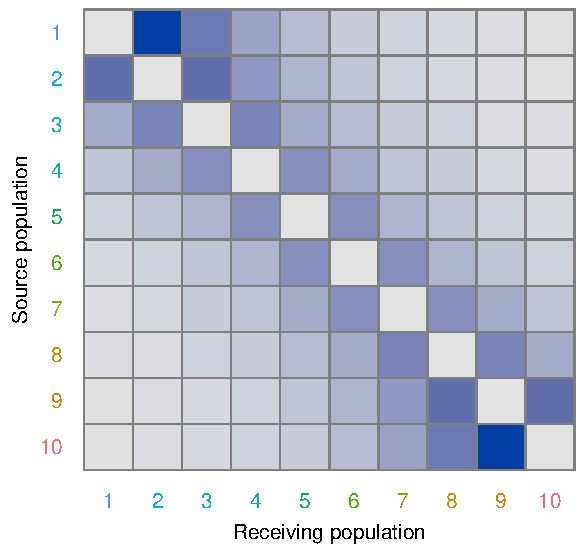
\includegraphics[width=4.0in]{../examples/figure/stray-matrix.pdf}
\caption{ An example straying matrix. The rows and columns represent different populations (indicated by population number). Dark blue indicates a high rate of straying and light blue indicates a low rate of straying.  The straying matrix is generated through equation \ref{eq:stray}.}
\label{f:stray}
\end{figure}

\clearpage

\begin{figure}[htbp]
\centering
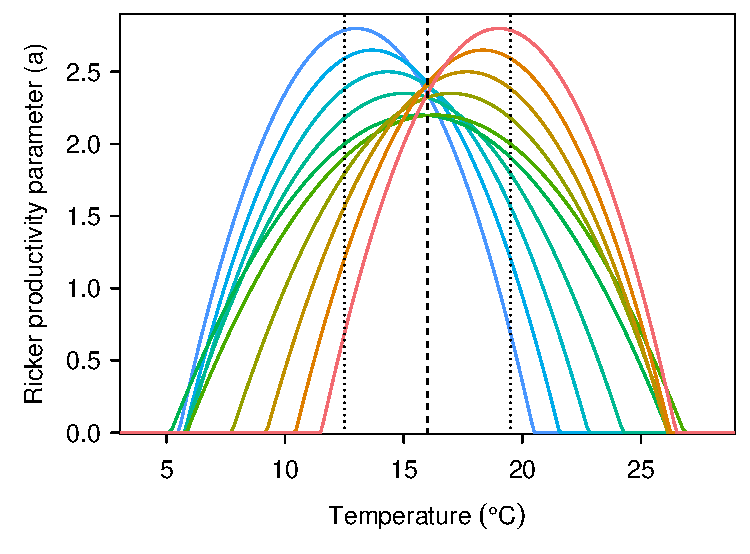
\includegraphics[width=4.5in]{../examples/thermal-curves.pdf}
\caption{The full range of environmental tolerance curves shown for 10 populations. The vertical dotted lines indicate the general range of environmental fluctuations in the main simulations, and the vertical dashed line indicates the mean environmental value in the main simulations.}
\label{f:all-curves}
\end{figure}

\clearpage

\begin{figure}[htbp]
\centering
\includegraphics[width=4.5in]{../examples/spatial-arma-sim.pdf}
\caption{Spatial and short-term environmental fluctuations}
\label{f:eg-sp-arma}
\end{figure}

\clearpage

\begin{figure}[htbp]
\centering
\includegraphics[width=4.5in]{../examples/spatial-linear-sim.pdf}
\caption{Spatial and long-term environmental fluctuations}
\label{f:eg-sp-linear}
\end{figure}

\clearpage

\begin{figure}[htbp]
\centering
\includegraphics[width=4.5in]{../examples/n-arma-sim.pdf}
\caption{Number and short-term environmental fluctuations}
\label{f:eg-n-arma}
\end{figure}

\clearpage

\begin{figure}[htbp]
\centering
\includegraphics[width=4.5in]{../examples/n-linear-sim.pdf}
\caption{Number and long-term environmental change}
\label{f:eg-n-linear}
\end{figure}

\clearpage

A placeholder: \citep{Schindler2010}

\bibliographystyle{apalike}

\bibliography{jshort,som}
